\raggedbottom
\chapter{Methods}\label{CHAPTER_Methods}
In this chapter, we describe the methods to study the structure and dynamics of water and aqueous electrolyte solutions.
DFTMD simulations are performed to calculate the theoretical VSFG spectra. 
Our motivations for adopting DFTMD simulations are manifold.
In general, DFTMD simulations have the following advantages: 
(1) structure and reactivity can be treated in a consistent way;
(2) efficient treatments of basis sets and long range interactions in the DFT do extend the simulation capabilities to 
thousands of atoms, i.e., it allows realistic models for interfaces;
(3) they provide information on the structural organization of the solvent at the interfaces. 
In particular, the interface of solutions contains a large number of water molecules and a HB network composed of H-bonds between them.
As Stillinger said, since H-bonding is the most important interaction in liquid water and since these interactions 
are cooperative, it is insufficient for the purposes of computer simulation to use the potential energy function for dimers alone\cite{Stillinger1980}.

The organization of this chapter is the following.
Paragraph \ref{section_AIMD} to \ref{section_BOMD} give an introduction to the basic ideas of the DFTMD as well as the BOMD we adopted.
Paragraph \ref{section_VDOS} and \ref{section_VSFG} introduce the analysis methods used in this thesis, including the method of calculating 
vibrational properties from velocity autocorrelation and the method of calculating VSFG spectra from the Velocity Auto-Correlation Function (VACF).
Paragraph \ref{section_SFG_Exp} includes the available experimental data for VSFG spectra of solution/vapor interfaces.

\section{Modeling interfaces with \abinitio molecular dynamics}\label{section_AIMD}
Modern theoretical methodology, aided by the advent of high speed computing, has advanced
to a level where the microscopic details of dynamical processes in condensed phases can be
treated on a relatively routine basis. One common theoretical approaches
for obtaining these microscopic details of the system is the MD simulations.
In the MD simulations, classical Newton equations of motion for
a system are solved numerically starting from a pre-specified initial state, and subject to a set of
boundary conditions appropriate to the problem. The MD methodology allows both equilibrium
thermodynamic and dynamical properties of a system at finite temperature to be computed,
while simultaneously providing a view of the microscopic motion of individual atoms
in the system\cite{Tuckerman2010}.

%[The reason to use  AIMD to simulate the water/vapor interface]
Despite the success of classical MD simulations, they  have some limitations. First, charges
are treated as static parameters, therefore electronic polarization effects are
not included.  The so-called polarizable models\cite{Rick94,SWR02,Lamoureux03}, in which charges 
and induced dipoles are allowed to fluctuate in a changing environment, 
have been proposed to overcome this problem. 
While having considerable success, they also have serious limitations, including a lack of transferability 
and standardization\cite{TME02}. Second, force fields assume a pre-specified connectivity among the atoms, therefore, they suffer
from an inability to describe chemical bond-forming and -breaking. This problem
can be treated using techniques such as the empirical valence
bond method\cite{AW80} or other semi-empirical approaches. Unfortunately, these methods are also not
transferable and, therefore, need to be reparametrized for each type of reaction and may end
up biasing the reaction path in undesirable ways.

To overcome these limitations of force field based approaches, \abinitio molecular dynamics (AIMD) simulation techniques\cite{DKR90,MCP92,Allen1993,MET96,MP97,DM00,RC02}
can be used. The AIMD simulation combines finite temperature dynamics with forces
obtained from electronic structure calculations performed ‘on the fly’ as the MD simulation
proceeds\cite{DM00}. Because the electronic structure is treated explicitly in the AIMD calculations,
many-body forces, electronic polarization and bond-forming and -breaking events are described
with the accuracy of the electronic structure representation. Moreover, the AIMD
method can be easily extended to incorporate nuclear quantum effects via the Feynman
path integral approach\cite{RPF65,RPF72}, leading to the \abinitio path integral technique\cite{DM96,MT96,DM99}.

The AIMD method have been used to study a wide variety of chemically
interesting problems in areas such as chemical reactivity, H-bonds for the interfacial structure, pKa,
and vibrational spectroscopy. The AIMD applications include calculations of the structure and dynamics of water and other H-bonded liquids, 
proton transport in aqueous and condensed phase environments, structure, proton order/disorder and dynamical properties of ice, structure of
liquid silicates and glasses, mechanisms of polymer knotting, Ziegler-Natta industrial catalysis
and other surface catalytic processes. 
More recently, the AIMD methods have started to impact the
biological sciences and have been applied in calculations of nuclear magnetic resonance chemical shifts in 
drug-enzyme complexes, structure of nucleic acids, exploration of the design of possible
biomimetics and structure, dynamics and binding mechanisms in myoglobin.
In many of these applications, new physical phenomena have been revealed, which could
not have been uncovered using empirical models, often leading to new interpretations of
experimental data and even suggesting new experiments to perform\cite{TME02}.

%[The reason to use the AIMD? ] 
%[How to model the water/vapor interface system? ]
To study the heterogeneous environment at water interface, the AIMD method is particularly suitable for the following reasons:
(1) The AIMD method is only relying on the atomic coordinates of the model system $\bf R$, and not on any adjustable parameter, 
i.e., the interatomic forces ${\bf F}_{\text{I}}=-\bigtriangledown_{{\bf R}_{\text{I}}}V({\bf R})$, where $V({\bf R})$ is the potential energy\cite{VKMP},
are determined using the first principle electronic structure methods on the fly; 
(2) New phenomena that are not foreseen before starting the simulation can simply happen if necessary.
Therefore, the AIMD method is also a good predictive tool. 
However, as a drawback, the AIMD simulations are expensive and can nowadays be performed on size-limited system of 100--1000 atoms for up to a few hundred ps. 

\section{Density functional theory} \label{section_DFT}
In most currently performed AIMD simulations, the dynamics is performed within the so-called Born-Oppenheimer (BO) approximation.
Since the mass of an electron is much smaller than that of any nuclei, there is a strong separation of timescales between the electronic and nuclear motion. 
We assume that the kinetic energy of nuclei is zero and their potential energy is constant in each moment of the dynamics.
Therefore, the electrons can be treated independently at constant nuclear coordinates $\bf R$.
Applying BO approximation, the potential energy $V(\bf R)$ is  written as
\begin{equation}
  V({\bf R})=\langle \Psi_0 | H_{\text{e}} | \Psi_0 \rangle + E_{I}({\bf R}),
\label{eq:BO}
\end{equation}
where $|\Psi_0\rangle$ is the ground state, 
$E_I({\bf R})$ is the energy of the nuclei,
and $H_{\text{e}}$ is the electronic many-body Hamiltonian, which depends on the electronic 
coordinates but parametrically on the nuclear degrees of freedom, 

After the BO approximation, a formidable task is to solve the electronic, non-relativistic, time independent many-body Sch\"{o}dinger equation
\begin{equation}
H_{\text{e}} |\Psi_0 \rangle = \epsilon_0({\bf R})|\Psi_0 \rangle.
\label{eq:SE}
\end{equation}
This is a high-dimensional eigenvalue problem, and it is still time consuming. 
One great solution to the electronic structure problem (to solve the electronic, non-relativistic, time independent many-body 
Sch\"{o}dinger equation) is the DFT\cite{HK64,KS65}.

DFT can be used to map the problem of a interacting electron gas onto that of a single particle in an effective non-local 
potential\cite{MCP92}. It provides a favorable compromise between computational cost and accuracy.

%[HK theorem]
Hohenberg and Kohn (HK) proved that the total energy of a many-electron system is a unique functional of the electron density $n(\bf r)$.
The first HK theorem proves that there exists a one-to-one correspondence between the ground state electronic density $n_0(\bf r)$ 
and an external potential $v(\bf r)$, i.e., the electron density  $n$ determines all
properties of a non-degenerate ground state of an atom or molecule (for a degenerate 
ground state the density $n$ determines the energy).
(If we want to solve variationally for the ground state energy of a system with $H=T + V_{ee}+\sum_{i=1}^N v(i)$) the 
HK theorem says that there exists a valid functional $Q[n]$ that delivers the sum of the electronic kinetic energy $T[n]$ 
and electron-electron repulsion energy $V_{ee}[n]$ of each trial electron density $n$\cite{Levy1979}.

The electronic density $n(\bf r)$ which depends on just 3 electronic degrees of freedom, become the central quantity in DFT 
in place of the complex $3N_{\text{e}}$-dimensional many-body wave-function.

The second HK theorem states that the total energy in the electronic density space satisfies
\begin{equation}
        E^{\text{DFT}}[n_0]= \psi_0  H_{\text{e}} \psi_0 \leq \psi' H_{\text{e}} \psi' =E^{\text{DFT}}[n'],
\label{eq:HK2}
\end{equation}
for which the equality holds if and only if $n_0=n'$ (variational principle).
One try to choose different $n$ to optimize $E^{\text{DFT}}[n]$, the quantum expectation value of $H_{\text{e}}[n]$, thus to determine $E^{\text{DFT}}[n_0]$, i.e.
\begin{equation}
E^{\text{DFT}}[n_0]= \min\limits_{\psi} \psi  H_{\text{e}} \psi  = \min\limits_{n}\psi[n]H_{\text{e}}[n]\psi[n] =\min\limits_{n}E^{\text{DFT}}[n],
\label{eq:var}
\end{equation}
Eq.\thinspace(\ref{eq:SE}) can be solved by iteratively diagonalizing $H_{\text{e}}[n]$ within a self consistent field (SCF) procedure.

%[The ground-state energy of a many-electron system as minimum of an energy functional]
Assuming atomic units and considering the physical relevant Coulomb interaction, the total Hamiltonian is 
\begin{align}        
        H_{\text{e}} =& \frac{1}{2}\sum_{i=1}^{N_{\text{e}}}\bigtriangledown_i^2 +\sum_{i<j}^{N_{\text{e}}}\frac{1}{|{\bf r}_i -{\bf r}_j|} +\sum_{I,i}^{N,N_{\text{e}}}\frac{Z_I}{|{\bf R}_I - {\bf r}_i|}   \nonumber \\
        =& {\hat{T}}+{\hat{U}}+{\hat{V}},
\label{eq:H}
\end{align}
where $Z_I$ is the atomic number of atom $I$, ${\hat{T}}$ is the operator of kinetic energy of electrons, ${\hat{U}}$ is the 
electron-electron interaction and  ${\hat{V}}=\sum_i v({\bf r}_i)$ is the electron-nuclei operator.

In DFT, we obtain the ground state energy of a many-electron system as minimum of an energy functional
\begin{equation}
E^{\text{DFT}}[n({\bf r})] = T[{n (\bf r)}] + U[n({\bf r})] + V[n(\bf r)].
\label{eq:asume}
\end{equation}
The next problem is how to provide an explicit form for the three terms appearing in Eq.\thinspace(\ref{eq:asume}). 
The solution is the Kohn-Sham approach to DFT. 
A reference system with the same electron density as the density for the full interacting system  and without electron electron repulsion is introduced. 
For such reference system, the kinetic energy functional is
\begin{equation}
        T_\text{s}[n({\bf r})]= - \frac{1}{2}\sum_{i=1}^{N_{\text{e}}}\int d{\bf r} \psi_i^*({\bf r})\bigtriangledown^2\psi_i({\bf r})
        = T_\text{s}[\{\psi_i[n({\bf r})]\}],
 \label{eq:kinetic_ks}
\end{equation}
and the electronic density can be written as 
\begin{equation}
n({\bf r})=\sum_{i=1}^{N_{\text{occ}}}f_i \psi_i({\bf r})\psi_i^*({\bf r}),
\end{equation}
in which $N_{\text{occ}}$ is the number of occupied orbitals and $f_i$ the occupation number of the $i$th state, so that
\begin{equation}
 \sum_{i=1}^{N_{\text{occ}}}f_i =N_{\text{e}},
\end{equation}
and $\psi_i({\bf r})$ is the wave-function of the $i$-th state. 

The total energy functional of the Kohn-Sham (KS) system is
\begin{align}
 E^{\text{KS}}[n({\bf r})]=&E^{\text{KS}}[\{\psi_i[n({\bf r})]\}]  \nonumber \\
        =&T_\text{s}[\{\psi_i[n({\bf r})]\}] +U_H[n({\bf r})] +V[n({\bf r})]+E_{\text{XC}}[n({\bf r})] \label{eq:T_s} \\
 =&-\frac{1}{2}\sum_{i=1}^N f_i \int d{\bf r} \psi_i^*({\bf r})\bigtriangledown^2\psi_i({\bf r})
 +\frac{1}{2}\int d{\bf r} \int d{\bf r}'\frac{n({\bf r})n({\bf r}')}{{\bf r}-{\bf r}'}  \nonumber \\
+&\int d{\bf r} v_{\text{ext}}({\bf r})n({\bf r}) + E_{\text{XC}}[n({\bf r})], \label{eq:E_KS}
 \end{align}
 where $ E_{\text{XC}}[n({\bf r})] \equiv (T[n({\bf r})] - T_\text{s}[\{\psi_i[n({\bf r})]\}])+(U[n({\bf r})]-U_H[n({\bf r})])$ 
 is the exchange and correlation (XC) energy functional and 
$v_{\text{ext}}=\delta V[n({\bf r})]/\delta n({\bf r})$ is the external potential. 
The energy functional $ E_{\text{XC}}[n({\bf r})]$ is the only unknown part of the total energy functional.
This definition of XC energy functional shows that a significant of part $E_{\text{XC}}$ is due to correlation effects 
of the kinetic energy, that is expressed explicitly only with the reduced 2-particle density matrix.

Directly minimizing Eq.\thinspace(\ref{eq:T_s}) is not straightforward because $T_\text{s}[\{\psi_i[n({\bf r})]\}]$ 
is an explicit orbital functional. However, it is more appropriate to
make $E_{\text{KS}} [\{\psi_i [n({\bf r})]\}]$ stationary by the following Euler-Lagrange equation.
It is possible to use the variational principle to derive the corresponding Euler-Lagrange equation of
the non- interacting system within the potential $v_{\text{ext}}$.
The KS scheme permits to map the full interacting many-body problem, with the electron-electron interaction $\hat U$
onto an equivalent fictitious single-body problem, with an effective potential operator 
$\hat V_{\text{KS}}=\hat U_s + \hat V_{\text{H}} + \hat V_{\text{XC}}$.

%\paragraph{Euler-Lagrange equation}
%[Hartree-Fock Approx.]
If we figure out a way to approximate the $V_{\text{XC}}$ accurately, we will have a much less demanding set of equations 
to solve than those of the true system\cite{Burke07}.
Using the variational principle is possible to derive the corresponding Euler-Lagrange equation of the reference 
system (non-interaction system) within the potential $v$.
To determine the set of wave-functions $\psi_i$ which minimize the KS energy functional , we can iteratively solve the equation
\begin{align}
  \bigl[T_\text{s}[n({\bf {r}})] +V_\text{H}[n({\bf{r}})] +V[n({\bf{r}})]+E_{\text{XC}}[n({\bf{r}})] \bigr]\psi_i({\bf{r}})=\varepsilon_i\psi_i({\bf{r}}), \label{eq:KSE}
\end{align}
where $\varepsilon_i$ is the eigenvalue of each equation, $V_\text{H}$ is the Hartree potential of the electrons:
\begin{align}
 V_{\text H} = e^2 \int\frac{n({\bf r})n({\bf r}') }{|{\bf r}- {\bf r}'|}d{\bf r} ',
 \end{align}
and the exchange and correlation potential
 \begin{align}
 V_{\text {XC}} = \frac{\delta E_{\text{XC}}[n({\bf r})]} {\delta n({\bf r}) }.
 \end{align}
Given the explicit form of the exchange and correlation functional $E_{\text{XC}}$, the exchange and correlation potential $V_{\text {XC}}$ can be determined, and thus electron density $n({\bf r})$. Thus the KS equation must be solved self-consistently.

The simplest density functional approximation is the Local Density Approximation (LDA). 
In LDA, the exchange and correlation energy of an electronic system is
\begin{equation}
E_{\text{XC}}[n({\bf r})]= \int\varepsilon_{\text{XC}}({\bf r}){n({\bf r})}d{\bf r},
\label{eq:E_XC}
\end{equation}
and
\begin{equation}
\frac{\delta E_{\text{XC}}[n({\bf r})]}{\delta n({\bf r})}=\frac{\partial n({\bf r})\varepsilon_{\text{XC}}({\bf r})}{\partial n({\bf r})},
\label{eq:delta_E_XC_2}
\end{equation}
where 
\begin{equation}
\varepsilon_{\text{XC}}({\bf r})= \varepsilon^{\text{hom}}_{\text{XC}}[n({\bf r})].
\end{equation}
The LDA is accurate for systems with slowly varying charge densities. 
It has a tendency to favor more homogeneous systems and over-binds solids and molecules. 
The dielectric and piezoelectric constant calculated from the LDA are approximately 10\% over estimated. 
The limitations of the LDA suggest that care must be taken into its applications. 
For example, the independent particle picture  breaks down in strongly correlated systems, where the LDA is very inaccurate. 
Furthermore, the LDA does not take into account variation of the electronic density and van der Waals interactions\cite{Burke07}, 
so it does not give a very accurate description of H-bonding.
H-bonding is essential for a correct description of water and interfaces 
with water, therefore, a functional beyond the LDA is needed in the description of hydrogen-bonded systems, including water.

For any density that varies sufficiently slowly, an expansion of a functional $f$ in gradients should have increasing
accuracy:
\begin{equation}
f[n]= \int d^3r [a n({\bf r})+b n({\bf r})|\nabla n({\bf r})|^2 + \cdots].
\label{eq:any_f}
\end{equation}
But the gradient expansion of the exchange-correlation energy does not always improve results, sometimes it leads to divergences.
Therefore, a more general approach which is called Generalised  Gradient Approximation (GGA) is considered. An approach to improve the 
LDA is to include gradient corrections , in which $E_{\text{XC}}$ is a functional of density and its gradient:
\begin{equation}
  E^{\text{GGA}}_{\text{XC}}[n({\bf r})] = \int \varepsilon_{\text{XC}}\bigl(n({\bf r})\bigr)n\bigl(F_{\text{XC}}[ n({\bf r}), |\nabla n({\bf r})| ]\bigr)d{\bf{r}},
\end{equation}
where $F_{\text{XC}}[n({\bf r})]$ is a correction chosen to satisfy conditions for $E_{\text{XC}}$. The XC energy depends locally on the
gradient of the density $\nabla n$ as well as the density $n$. There are several forms of the GGAs. 

The GGA is usually the best compromise between speed and accuracy in large systems. For solids, the most commonly used functional
with the GGA is the one proposed by Perdew, Burke and Ernzherhof (PBE)\cite{PBE96}.
Another popular GGA functional is the BLYP functional.  
The electron densities of electric dipole and quadruple moments are not uniform in space.
Physically, GGAs include information on the spatial variation in the electron densities,
and thus they can create functionals with better flexibility to describe dipole and quadruple moments. 
Therefore, GGAs generally describe the dipole and quadruple moments of the monomer quite well. 
However, they somewhat overestimate polarizabilities, the predicted dipolar 
polarizability (also called dipole polarizability) being typically 10\% too large.

%[Dispersion Forces]
Dispersion is a general term referring to weak, long-range correlations in electronic structure. It includes van der Waals interactions,
which originates from the coupling of the electric field generated by fluctuations in the electronic density at position $\bf{r}$ 
in the system with the density at another point $\bf{r'}$\cite{Zeiss1977,Kohanoff06}. These interactions are not well modelled by any mean-field level of theory, 
the \abinitio wave-function theory such as second-order M{o}ller-Plesset perturbation theory (MP2), 
or standard DFT functionals, eg. LDA, GGAs, etc. 
The mean-field theory does not include the electron correlation effect, MP2 theory usually overestimate the binding energies 
and underestimates intermolecular equilibrium distances, and all the gradient corrected DFT are unable to describe dispersion 
interactions,because they can not describe the long-range electron correlation.
In the last two decades, a series of empirical corrections have been proposed which can improve the structural properties 
without more computational cost\cite{WuX01,WuQ02,Zimmerli04,Grimme04,Grimme06,Grimme07,Grimme10}.
Among such empirical approaches we  choose the DFT-D3 correction which can be used in our application to interfaces with water\cite{Grimme10,Klimes2012}.

%Detail of D3
In the DFT-D3 correction, also used in this thesis, the input parameters are cutoff radii and dispersion coefficients, and they can be calculated by 
KS-DFT methods using extended atomic orbital basis sets. The use of structure dependent dispersion coefficients, 
i.e., functional coordination number, to interpolate between dispersion coefficients of atoms in different chemical environments, 
increases the accuracy.  Moreover, no atom connectivity information is required and all the properties are calculated only 
from Cartesian coordinates and atomic numbers\cite{Grimme10}.

If the three-body nonadditivity terms are considered, as well as the pairwise terms, the total energy is given by 
\begin{equation}
    E_{\text{DFT}} = E_{\text{KS-DFT}}+E_{\text{disp}}^{(2)}+E_{\text{disp}}^{(3)},
\label{eq:e_dftd3}
\end{equation}
where $E_{\text{KS-DFT}}$ is the usual self-consistent KS energy obtained from the chosen density functional, $E_{\text{disp}}^{(2)}$ is the empirical two-body  dispersion correction term and $E_{\text{disp}}^{(3)}$ is the three-body nonadditivity term. $E_{\text{disp}}^{(2)}$ is given by
\begin{equation}
    E_{\text{disp}}^{(2)} = \sum_{\text{AB}}\sum_{n=6,8,10,\cdots}s_n\frac{C_n^{\text{AB}}}{R_{\text{AB}}^n}f_{\text{dmp},n}(r_{\text{AB}}),
    \label{eq:e_disp_2}
\end{equation}
where $\sum\limits_{\text{AB}}$ denotes the sum over all atom pairs in the system\cite{Zeiss1977},
$C_n^{\text{AB}}$ is the averaged $n$-order dispersion coefficients ($n=6{,}8{,}10{,}\cdots$) for atom pair AB,
$r_{\text{AB}}$  is the inter-nuclear distance of atom pair AB,
and $f_{\text{dmp},n}(r_{\text{AB}})$ is the damping function used to avoid near-singularities for small distance $R$  between nuclei.
The damping function in Eq.\thinspace(\ref{eq:e_disp_2}) is given by 
\begin{equation}
    f_{\text{dmp},n}(r_{\text{AB}}) = \frac{1}{1+6(r_{\text{AB}}/(s_{r,n}R_0^{\text{AB}}))^{-\alpha_n}},
    \label{eq:e_damping}
\end{equation}
where $s_{r,n}$ is the order-dependent scaling factor of the cutoff radii $R_0^{\text{AB}}$, 
which is the most important parameter that has to be adjusted for each density functional 
and $\alpha_n$ is a parameter which can be adjusted manually such that the dispersion correction is 
smaller than 1\% of max($|E_{\text{disp}}|$) for typical covalent bond distances.
In Ref.\cite{Grimme10} $s_{r,6}$ is optimized by a least-squares fitting procedure and $s_{r,8}$ is fixed to 1 for all density functionals.

The leading non-additive dispersion term for three atoms A, B and C is
\begin{equation}
    E_{\text{disp}}^{(3)} =\frac{C_9^{\text{ABC}}(3\text{cos}\theta_a\text{cos}\theta_b \text{cos}\theta_c+1)}{(r_{\text{AB}}r_{\text{BC}}r_{\text{CA}})^2},
\label{eq:e_ABC}
\end{equation}
where $\theta_a$, $\theta_b$ and $\theta_c$ are the internal angles of the $\Delta$ABC,
and $C_9^{\text{ABC}}$ is the triple-dipole constant defined by 
\begin{equation}
  C^{\text{ABC}} =\frac{3}{\pi}\int_0^{\infty}\alpha^{\text{A}}(i\omega)\alpha^{\text{B}}(i\omega)\alpha^{\text{C}}(i\omega),
\label{eq:C_ABC}
\end{equation}
which can be approximated by a geometric mean
\begin{equation}
C^{\text{ABC}} \approx -\sqrt{C_6^{\text{AB}}C_6^{\text{AC}}C_6^{\text{BC}}},
\label{eq:C_ABC_approx}
\end{equation}
since the total three-body contribution is typically 5--10\% of $E_{\text{disp}}=E_{\text{disp}}^{(2)}+E_{\text{disp}}^{(3)}$.
%
\section{Born-Oppenheimer molecular dynamics}\label{section_BOMD}
%[Ehrenfest MD, CPMD and BOMD]
In computational material science, the most popular AIMD simulation methods are the Born-Oppenheimer MD (BOMD) and Car-Parrinello MD (CPMD) methods. 
In the BOMD, the potential energy $E[\{\psi_i\};\bf{R}]$ is minimized at each MD step with respect to $\{\psi_i({\bf r})\}$  under the orthonormality condition
\begin{equation}
\langle\psi_i({\bf{r}})|\psi_j({\bf r})\rangle=\delta_{ij}.
\label{eq:e_XC}
\end{equation}
Thus the Lagrangian density is 
\begin{align}
L_\text{BO} (\{\psi_i\}; {\bf R}_{I})=&\frac{1}{2}\sum^N_{I=1}M_{\text{I}}\dot{\bf R}^2_{I} - {\text{min}}_{\{\psi_i\}}E[\{\psi_i\};{\bf R}_{I}] \nonumber \\
             +& \sum_{i,j}\Lambda_{ij}(\langle\psi_i|\psi_j\rangle-\delta_{ij} ),
\label{eq:L_BO}
\end{align}
in which $\Lambda$ is the Hermitian Lagrangian multiplier matrix. By the Euler-Lagrange equations one obtains the equations of motion
\begin{align}
     M_{I}{\bf \ddot{R}}_I =& -\nabla_{R_I} \bigl[ {\text{min}}_{\{\psi_i\}}E[\{\psi_i\};{\bf R}_I] |_{\langle\psi_i|\psi_j\rangle=\delta_{ij} }\bigr]\nonumber \\
     =&-\frac{\partial E}{\partial {\bf R}_{I}}  + \sum_{i,j}\Lambda_{ij}\frac{\partial}{\partial {\bf R}_I}\langle\psi_i|\psi_j\rangle \nonumber \\
     -&2\sum_i \frac{\partial \langle\psi_i|}{\partial {\bf R}_I}\biggl(\frac{\delta E}{\delta\langle\psi_i|}-\sum_j \Lambda_{ij}|\psi_j\rangle\biggr) 
\label{eq:LEE_BO}
\end{align}
The term $-\frac{\partial E}{\partial {\bf R}_{\text{I}}}$ is the Hellmann-Feynman force, and the term $\sum_{i,j}\Lambda_{ij}\frac{\partial}{\partial {\bf R}_{\text{I}}}\langle\psi_i|\psi_j\rangle$, i.e., the wave-function force $F_{\text{WF}}$\cite{Pulay69}, is a constraint force due to the orthonormality constraint. The last term comes from the fact that there is always an implicit dependence on the atomic positions through the expansion coefficient $c_{ij}({\bf r})$ that is defined by 
\begin{equation}
\psi_i({\bf r})=\sum_j c_{ij}({\bf r})\phi_i({\bf r}),
\label{eq:linear_combination}
\end{equation}
where the KS orbitals are assumed to be real.

The CPMD is an alternative method to the BOMD, which includes the 
electrons in a single state\cite{CP}. In the CPMD, a coupled electron-ion dynamics is performed.
The CP Lagrangian is 
\begin{align}
L_{\text{CP}} (\{\psi_i\}; {\bf R},\dot{{\bf R}}) =& \frac{\mu}{2}\sum_i\langle\dot{\psi}_i|\dot{\psi}_i\rangle +  \frac{1}{2}\sum^N_{I=1}M_{\text{I}}\dot{\bf R}^2_{\text{I}}  - E[\{\psi_i\};{\bf R}] \nonumber \\
   +& \sum_{i,j}\Lambda_{ij}(\langle\psi_i|\psi_j\rangle -\delta_{ij} ),
\label{eq:L_CP}
\end{align}
where the electronic degrees of freedom carries a fictitious mass parameter $\mu$, and are characterized by orbital velocities 
$\{\dot{\psi}_i\}$.  Applying the Euler-Lagrangian equations leads the equations of motion:
\begin{align}
  M_{\text{I}}\ddot{\bf R}_{\text{I}} =& -\nabla_{R_{\text{I}}} \bigl[E[\{\psi_i\};{\bf R}]|_{\langle\psi_i|\psi_j\rangle=\delta_{ij} }\bigr]\nonumber \\
  =&-\frac{\partial E}{\partial {\bf R}_{\text{I}}}  + \sum_{i,j}\Lambda_{ij}\frac{\partial}{\partial {\bf R}_{\text{I}}}\langle\psi_i|\psi_j, \rangle\\ 
  \mu\ddot{\psi}_i({\bf r},t) =& -\frac{\partial \langle\psi_i|}{\partial {\bf R}_{\text{I}}}\biggl(\frac{\delta E}{\delta\langle\psi_i|} + \sum_j \Lambda_{ij}|\psi_j\rangle\biggr)\nonumber \\
  =& -\hat{H}_{\text{e}}\langle\psi_i| + \sum_j \Lambda_{ij}|\psi_j\rangle,
\label{eq:LEE_CP}
\end{align}
where $-\delta E/\delta\psi_i$ are the electronic forces to propagate the electronic degrees of freedom in time 
within a fictitious Newtonian dynamics.  No SCF cycle is required to quench the electrons to the Born-Oppenheimer surface and 
to force them to evolve adiabatically with respect to the nuclei.

%[A proper choice of the ficticious mass $\mu$]
To ensure the adiabatic energy-scale separation of the nuclear and the electronic degrees of freedom, i.e. 
to prevent energy transfer between them, the highest nuclear phonon frequency  $\omega_{\text{I}}$ must be 
much smaller than the lowest electronic phonon frequency $\omega_{\text{e}}$. The condition $\omega_{\text{I}} \ll \omega_{\text{e}}$ 
is ensured by a proper choice of the fictitious mass $\mu$. The fictitious mass determines the computational accuracy.  

%BOMD or CPMD? 
Which method is to favor depends largely on the definition of accuracy, as well as on the particular application.
In the applications in this thesis, we use the BOMD method, as implemented in CP2K package\cite{CP2K,Kuehne2020}. 
In the BOMD  
(1) the nuclear positions are propagated in time followed Newton's equations of motion with the electronic ground state energy as the potential energy surface; 
(2) the time evolution of the atomic coordinates is performed with the velocity Verlet algorithm\cite{FS2002}.

%[The integration time step problem]
Since there is no explicit electron dynamics, the maximum integration time step is simply given by the one intrinsic 
to nuclear motion, i.e., $\tau_{e}^{\text{BO}}\approx\tau_{\text{n}}$. 
In BOMD, the time step can be even larger if the nuclear dynamics becomes fairly slow\cite{GK93}. 
But in order to resolve vibrations in molecular systems, the time step is decreased to less than 1 fs in this thesis\cite{DM00}.
%
\section{Vibrational density of states}\label{section_VDOS}
To obtain the vibrational properties of a molecular system, it is possible to use the VACFs,
as calculated from the AIMD trajectories.
The obtained Vibrational Density of States (VDOS) can 
provide information on the local environment of the water molecules' OH-stretching mode. 
For a system comprised of $N$ atoms, the velocity ACF $C(t)$ for a molecule is\cite{MTD,JMD,TI07} 
\begin{equation}
C(t)=\frac{\langle\sum^{N}_{i=1}{\bf{v}}_i(t)\cdot{\bf{v}}_i(0)\rangle}{\langle\sum^{N}_{i=1}{\bf{v}}_i(0)\cdot{\bf{v}}_i(0)\rangle},
\label{eq:Ct3s}
\end{equation}
where $\langle\dots\rangle$ denotes the average over starting times, $t$ is the time interval, and ${\bf{v}}_i$ denotes 
the velocity of the $i$-th atom. The VDOS $g(\nu)$ for selected atoms, which is a function of the vibrational frequency $\nu$ 
of atoms, is expressed in terms of the Fourier Transform (FT) of the velocity ACF of the atoms\cite{MPA86}.
In equilibrium, $C(-t)=C(t)$, and $g(\nu)$ is a real function, i.e., 
\begin{equation}
g(\nu)= \sqrt{\frac{2}{\pi}}\int^{\infty}_{0}\text{d}t \text{cos}(2\pi\nu{t})C(t).
\label{eq:f_omega2}
\end{equation}
Single components of the VACFs can also be calculated. For example in the case of an interface it may be of interest to look at 
$z$-component (where $z$ is the direction perpendicular to the Gibbs interface),
we can calculate the FT $g_z(\nu)$ of the auto-correlation function of the vertical component of atomic velocity. 
$g_z(\nu)$ can be calculated by Eq.\thinspace(\ref{eq:f_omega2}) if we replace $C(t)$ by 
\begin{equation}
C_z(t)=\frac{\langle\sum^{N}_{i=1}{v_{i,z}(t){v_{i,z}(0)\rangle}}}{\langle\sum^{N}_{i=1}{\bf{v}}_i(0)\cdot{\bf{v}}_i(0)\rangle},
\label{eq:ACN}
\end{equation}
where $v_{i,z}$ is the vertical component of the velocity of the $i$-th atom.
The VDOS $g_z(\nu)$ for water molecules is used to extract the O-H stretch along the vertical direction to the interface. 

\section{Calculation of VSFG spectroscopy for interfaces}\label{section_VSFG}
%SFG calculation and measurement
%[Introduction of the VSFG spectroscopy]
As introduced in Chapter \ref{CHAPETR_1}, the VSFG spectroscopy is a powerful tool for extracting structural and dynamical information
on surfaces and interfaces.
It can be applied to any interface as long as light can reach it, also including liquid/metal interfaces\cite{Harris90,Harris90b,DaiHL95,Halevi96,Wieckowski99} 
and buried interfaces\cite{Chen99,Chen07};
It can probe liquid interface with molecular sensitivity\cite{Khatib16,Khatib16b,Khatib2017}.
Therefore, the VSFG spectroscopy can yield structural information about solution/vapor interfaces which could not be obtained with other techniques.

\subsection{Nonlinear susceptibility of solution/vapor interfaces}
% [Aim of VSFG simulations and VSFG theory]
%[
%    [PUT ELSEWHERE: this part is FOR introducing VSFG tech] Experiments required theoretical modeling in order to dissect the experimental results, and to rationalize the different factors that contribute to the interfacial properties.
%Perry et al.\cite{Perry03} developed a method to compute the VSFG spectrum from instantaneous normal modes (INM), 
%as well as a time correlation function method. They are based on classical MD simulations.
%]
\paragraph{VSFG}
The VSFG is a coherent nonlinear optical process in which incident laser beams with frequency and wave vector 
($\omega_1, {\bf k}_1$) and ($\omega_2, {\bf k}_2$) produce a signal with frequency and wave vector
($\omega_1+\omega_2, {\bf k}_1+{\bf k}_2$ ) (Fig.\thinspace\ref{fig:sfg_1a}). 
In this process, the fields arise from the polarization induced over a macroscopically large volume superposition coherently.
%
%\paragraph{Vibrational Resonances and Non-resonances}
The VSFG signal intensity is proportional to the square of the resonant and non-resonant terms:
\begin{align}
  &I_{\text{SFG}}(\omega) \varpropto |\chi^{(2)}(\omega)|^2 \nonumber \\
  &=|\chi^{(2),\text{R}}(\omega)+\chi^{(2),\text{NR}}(\omega)|^2,
\label{eq:I_SFG}
\end{align}
where $\chi^{(2)}$ is a third-rank tensor called second-order nonlinear susceptibility, or hyperpolarizability for a molecule\cite{Morita2018-page2},
and it is responsible to the VSFG process. 
$\chi^{(2),\text{R}}$ is the vibrationally resonant term, while $\chi^{(2),\text{NR}}$ is the nonresonant term.
\begin{figure}[h]
\centering
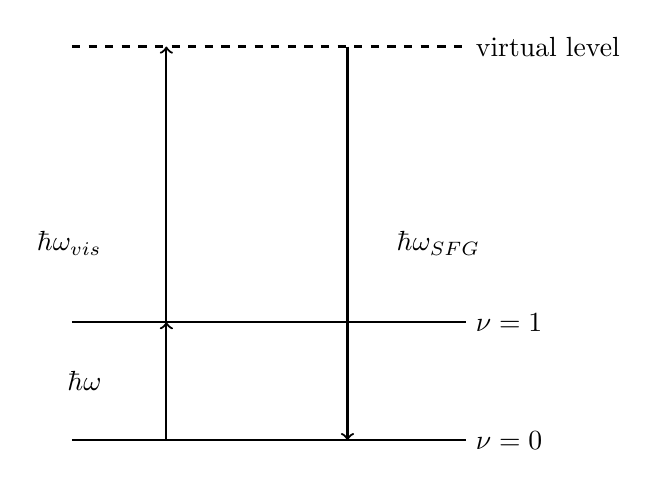
\begin{tikzpicture}[help lines/.style={thin,draw=black!50}]
%%\draw[help lines] (0,0) grid (4,4);
\draw [-, thick] (0,0) -- (5,0) node [anchor = west] {$\nu =0$};
\draw (0.5,0.75) node [anchor = east] {$\hbar\omega$};
\draw [-, thick] (0,1.5) -- (5,1.5) node [anchor = west] {$\nu = 1$};
\draw (0.5,2.5) node [anchor = east] {$\hbar\omega_{\text{vis}}$};
\draw [-, thick,dashed] (0,5) -- (5,5) node [anchor = west] {virtual level};
\draw (4.0,2.5) node [anchor = west] {$\hbar\omega_{\text{SFG}}$};
\draw [->, thick] (1.2,0) -- (1.2,1.5);
\draw [->, thick] (1.2,1.5) -- (1.2,5);
\draw [->, thick] (3.5,5) -- (3.5,0);
\end{tikzpicture}
\caption{The schematic diagram of the VSFG process which involves IR and Raman transitions. The $\nu =0$, $\nu=1$ levels denote the ground and the first excited state of the oscillator\cite{Gang202104}, respectively.
 The dashed line denotes a virtual electronic state in the Raman transition.
}\label{fig:sfg_1a} 
\end{figure}
%
Because experiments usually employed visible and the VSFG frequencies are far from resonant 
conditions, $\chi^{(2),\text{NR}}$ can be considered totally off-resonant and therefore 
insensitive to the laser beams' frequencies involved. Therefore, we can neglect the 
frequency dependence of the non-resonant term.
The molecular information is contained in the resonant signal. The resonant susceptibility $\chi^{(2),\text{R}}(\omega)$ is given by 
\begin{equation}
  \chi_{\eta\xi\kappa}^{(2),\text{R}}(\omega)=\frac{-i}{\hbar}\int_0^\infty dt e^{i\omega t} \text{Tr}{[\rho,\mu_\kappa]\alpha_{\eta\xi}(t)},
\label{eq:chi_R}
\end{equation}
where the index $\eta$, $\xi$ and $\kappa$ are one of $x, y$ and $z$ labels of the laboratory coordinate frame.
In Eq.\thinspace(\ref{eq:chi_R}) $\rho=e^{-\beta H}/Z$ for a system with Hamiltonian $H$ and partition function $Z$ at reciprocal temperature $\beta=1/k_BT$;
$\mu_\kappa$ is the $\kappa$-th component of the system electric dipole and ${\alpha_{\eta\xi}}$ is the $\eta\xi$-th component of the polarizabiltiy tensor\cite{1995SM}.
Besides the vibrational resonance, $\chi^{\text{(2),R}}$, which reflects the vibrational and orientational characteristics of the surface species, 
the VSFG signal also includes the contribution from the non-resonant signal background $\chi^{\text{(2),NR}}$, 
due to static hyperpolarizability of the interface itself\cite{Che2012}.  
For example, there are strong non-resonant second-order nonlinear responses\cite{Pradier11,Vanselow2012,Wieckowski99} of the interface in the case of some metal(-oxide). 
Generally, experiments employ visible light and VSFG frequencies far from resonant conditions, therefore, the non-resonant 
term $\chi^{\text{(2),NR}}$ is approximately off-resonant to the light frequencies involved\cite{Morita02}.
%Neglecting the frequency dependence of the nonresonant term $\chi^{\text{(2),NR}}$ is usually a good approximation. 

\paragraph{Microscopic expression of molecular hyperpolarizability} 
As the electric field is increased, the description of the induced dipole moment 
$\boldsymbol \mu$ should include the normally insignificant nonlinear terms. We can express the induced dipole moment as
\begin{equation}
  {\boldsymbol \mu} = {\boldsymbol \mu}_0 +\alpha {\bf E} + \beta {\bf E E}.
\label{eq:induced_mu}
\end{equation}
%or
%\begin{equation}
%  \mu_i = (\mu_0)_i +\alpha_i  E_i + \beta_{ijk}E_j E_k + \cdots.
%\label{eq:induced_mu}
%\end{equation}
The VSFG spectra are determined by the frequency-dependent hyperpolarizability in molecular level description. 
The frequency-dependent hyperpolarizability can be expressed as a sum of resonant and non-resonant terms:
\begin{equation}
\beta_{\eta\xi\kappa}(\omega_{\text{SFG}},\omega_{\text{vis}},\omega)=\beta_{\eta\xi\kappa}^{\text{R}}+\beta_{\eta\xi\kappa}^{\text{NR}},
\label{eq:beta}
\end{equation}
where $\eta$, $\xi$ and $\kappa$ are space-fixed axes.
The resonant term of the frequency-dependent hyperpolarizability is 
\begin{equation}
  \beta_{\eta\xi\kappa}^{\text{R}}(\omega_{\text{SFG}},\omega_{\text{vis}},\omega)=\sum_{v',v}\frac{\langle v|\alpha_{\eta\xi}|v'\rangle\langle v'|\mu_{\kappa}|v\rangle}{(\omega_{v'}-\omega_v)-\omega-i\gamma_{v'v}}\rho_v,
\label{eq:beta_R}
\end{equation}
where the subscripts $\eta$, $\xi$ and $\kappa$ denote body-fixed axes,
$\omega_{v'}-\omega_v$ is the vibrational energy gap, 
$\rho_v$ is the thermal distribution function of the initial vibrational states $v$,
$\alpha_{\eta\xi}$ is the $\eta\xi$-th component of the molecular dipole polarizability,
$\mu_{\kappa}$ is the $\kappa$-th component of the molecular dipole moment,
and $\gamma_{v'v}$ is the damping rate.
Since  
(see Appendix \ref{calculation_of_chi}) 
\begin{align}
\int_0^\infty dt e^{-it[(\omega_{v'}-\omega_v)-\omega-i\gamma_{v'v}]}=\frac{-i}{(\omega_{v'}-\omega_v)-\omega-i\gamma_{v'v}},
\label{integral_identity1a}
\end{align}
we can rewrite Eq.\thinspace(\ref{eq:beta_R}) as 
\begin{align}
  \beta_{\eta\xi\kappa}^{\text{R}}&=i\int_0^\infty dt \sum_{v'v}e^{-i[(\omega_{v'}-\omega_v)-\omega-i\gamma_{v'v}]t} \langle v|\alpha_{\eta\xi}|v'\rangle\langle v'|\mu_{\kappa}|v\rangle \rho_v \nonumber\\
   &=i\int_0^\infty dt \sum_{v'v}e^{i\omega t} \langle v|e^{iHt}\alpha_{\eta\xi}e^{-iHt}|v'\rangle\langle v'|\mu_{\kappa}|v\rangle \rho_v \nonumber\\
   &=i\int_0^\infty dt e^{i\omega t} \langle\alpha_{\eta\xi}(t)\mu_{\eta\xi}(0)\rangle,
\label{eq:beta_R_b}
\end{align}
where $H$ is the Hamiltonian of the system without external field. 
Eq.\thinspace(\ref{eq:beta_R_b}) indicates that the resonant term $\beta_{\eta\xi\kappa}^{(2),\text{R}}$ is the FT 
of the quantity $\langle\alpha_{\eta\xi}(t)\mu_{\kappa}(0)\rangle$, i.e., the ensemble average of the time correlation function $\alpha_{}(t)\mu_{r}(0)$.
The damping rate $\gamma_{v'v}$ is not explicitly included in Eq.\thinspace(\ref{eq:beta_R_b}), because the dephasing is incorporated in the time development of the off-diagonal matrix elements 
of $\alpha_{\eta\xi}(t)$ and $\mu_{\kappa}(0)$.

The tensor elements $\chi^{(2),R}_{\eta\xi\kappa}$ is microscopically represented as the average sum of first-order hyperpolarizability of the constituent molecules $\beta$ in the space-fixed frame
\begin{align}
  \chi^{(2),R}_{\eta\xi\kappa} = \langle \sum_i^N \sum_{pqr} D_{\eta p}(\Omega_i) D_{\xi q}(\Omega_i) D_{\kappa r}(\Omega_i) \beta_{pqr}\rangle
\label{average_sum}
\end{align}
where $D(\Omega_i)$ is the direction cosine matrix of the $i$-th molecule, projecting $\beta$ onto the space-fixed frame\cite{Morita2000}.

%and evaluate it with the static hyperpolarizability, which can be calculated by an \abinitio Molecular Orbital (MO) package\cite{Morita02}, 
%\begin{equation}
%        \beta_{\eta\xi\kappa}^{\text{NR}}=\sigma\beta_{\eta\xi\kappa}^{\text{static}},
%\label{eq:beta_NR}
%\end{equation}
%where $\sigma$ is the symmetry number among the indices $\eta$, $\xi$ and $\kappa$.
%\paragraph{Derive the value of $\sigma$}
%The frequency-dependent hyperpolarizability, $\beta(\omega_1,\omega_2,\omega_3)$, satisfies the following equation 
%\begin{equation}
%\label{eq:beta_condition}
%        P_p(\omega_1)=\sum_q\alpha_{pq}(\omega_1)E_q(\omega_1)+\sum_{qr}\beta_{pqr}(\omega_1,\omega_2,\omega_3)E_q(\omega_2)E_r(\omega_3)+\cdots
%\end{equation}
%where the suffices $p$, $q$ and $r$ range over $x$, $y$ and $z$, and $P_p(\omega_1)$ is the induced dipole moment at frequency $\omega_1$. The static polarizability and hyperpolarizability are defined as 
%\begin{equation}
%        \alpha_{pq}^{\text{static}}=(\frac{\partial P_p}{\partial E_q})_{E=0},\ \
%        \beta_{pqr}^{\text{static}}=(\frac{\partial^2 P_p}{\partial E_q \partial E_r})_{E=0}
%\label{eq:beta_condition}
%\end{equation}
%and thus the dipole moment in a static external electric field is expressed as 
%\begin{equation}
%        P_p^{\text{static}}=(P_p)_{E=0}+\sum_q\alpha_{pq}^{\text{static}}E_q+\frac{1}{2}\sum_{qr}\beta_{pqr}^{\text{static}}E_qE_r+\cdots,
%\label{eq:static_dipole_moment}
%\end{equation}
%where $(P_p)_{E=0}$ is the permanent dipole moment. From Eq. (\ref{eq:beta_condition}) and Eq. (\ref{eq:static_dipole_moment}), we obtain $\sigma=1/2$ in Eq. (\ref{eq:beta_NR}).

\paragraph{The Fresnel Factors}
Because of screening and dipole-dipole coupling, the local electric fields felt by molecules is different from the macroscopic fields\cite{Vanselow2012}. 
The VSFG signal depends on the magnitude of the local electric fields of the interacting optical beams at the interfaces. 
While the magnitude of the local electric fields is related to both the intensity of the incident beams and the linear refractive indices 
of the different layers (bulk) of the sample\cite{Khatib16}. The Fresnel coefficients define the magnitude of the electric fields at the interface. 
Therefore, to find out the magnitude of the local electric fields, we need to evaluate the Fresnel factors. 
The VSFG intensity $I_{\text{SFG}}$, is proportional to the intensities of the incident visible and infrared beams, $I_{\text{vis}}$, $I$, 
and to the square of the second-order nonlinear susceptibilities,
$\chi_{\eta\xi\kappa}^{(2)}(\omega_{\text{SFG}})$, of the interface:
\begin{equation}
        \chi_{\eta\xi\kappa}^{(2)}(\omega_{\text{SFG}})\propto|\sum_{\eta,\xi,\kappa}L_{\eta\eta}(\omega_{\text{SFG}})\chi_{\eta\xi\kappa}^{(2)}(\omega_{\text{SFG}})L_{\xi\xi}(\omega_{\text{vis}})L_{\kappa\kappa}(\omega)|^2\text{sec}^2(\theta_{\text{SFG}})I_{\text{vis}}I
\label{eq:chi}
\end{equation}
where $\eta$, $\xi$, $\kappa$ are the Descartes coordinates of the reference frame;
$\omega_{\text{SFG}}=\omega_{\text{vis}}+\omega$ is the frequency of VSFG beam; 
$L_{\eta\eta}$, $L_{\xi\xi}$ and $L_{\kappa\kappa}$ are the Fresnel coefficients; 
$\theta_{\text{SFG}}$ is the reflected angle of VSFG beam with respect to the normal 
direction in the medium.

\subsection{VSFG spectra from velocity auto-correlation functions}
%To construct SFG spectrum of O-H stretching at the water/vapor interface and to ascertain the molecular origin of SFG spectrum, 
%quantum corrected time correlation function \cite{Morita02,Morita04} and instantaneous normal mode (INM) methods are used 
%by Perry and coworkers.\cite{Perry03} 
%For  water/vapor interface, the INM SFG spectrum is in agreement with the time correlatin function SFG spectrum. 
%This implies that motional narrowing effects play little role  in the interfacial line shape. The Shen group suggests that 
%the motional narrowing effects may be significant in the SPS geometry, where the "free O-H" stretching peak is greatly diminished.\cite{WeiX02}
%========================
%\section{solutions}
%Here we discuss the calculation of nonlinear susceptibility of water molecules at liquid/vapor interfaces.
%The SFG spectrum is proportional to the square of the nonlinear susceptibility of water molecules at the water/vapor interface. \cite{QD94}  
%Details:
This paragraph gives the derivation an expression for the calculation of the sum frequency generation spectra of water interfaces that is
based on the projection of the atomic velocities on the local normal modes, such an approach permits one to obtain the VSFG signals from suitable
VACFs, reducing the computational cost to that of the accumulation of a molecular dynamics trajectory, and therefore cutting 
the overhead costs associated with the explicit calculation of the dipole and polarizability tensor. Moreover, the method permits to interpret 
the peaks in the spectrum in terms of local modes.
The components of the resonant term $\chi^{\text{(2),R}}_{\eta\xi\kappa}$ of the second order susceptibility can be calculated 
according to the classical formula\cite{Morita02,Morita2008,Nihonyanagi2011}
\begin{align}
  \chi^{\text{(2),R}}_{\eta\xi\kappa}&=\frac{-i}{k_{\text{B}}T \omega} \int_0^\infty dt e^{i\omega t}\left\langle \dot{A}_{\eta\xi}(t) \dot{M}_{\kappa}(0)\right\rangle 
 \label{eq:chi}
\end{align}
%\begin{align}
% \chi^{(2)}_{XXZ,R}&=\frac{i}{k_BT \omega} \sum\limits_j \int_0^\infty dt e^{i\omega t} \left \langle \frac{\partial A_{XX}}{\partial r_j} \frac{\partial M_Z}{\partial r_j}  \dot{r}_j(0) \dot{r}_j(t) \right\rangle
% \label{eq:chi2}
% \end{align}
where $k_{\text{B}}$ is the Boltzmann constant, $\omega$ is the frequency of the IR beam, ${\bf M}$ (${A}$) is the dipole 
moment (dipole polarizability) of the system, and $\left\langle\dots\right\rangle$ denotes the average over all starting time points. 
%The derivation of Eq.\thinspace(\ref{eq:chi}) is given in Appendix \ref{calculation_of_chi}.
 
 The total dipole moment and dipole polarizability derivatives for the system can be expressed in terms of the water and bond contributions:
\begin{align}
 \dot{A}&=\sum_{i=1}^N \sum_{\epsilon}\dot{\alpha}^{i,\text{l},\epsilon} \\ 
 \dot{{\bf M}}&=\sum_{i=1}^N \sum_{\epsilon}\dot{\mu}^{i,\text{l},\epsilon} 
 \label{eq:A-M}
\end{align}
where ${\mu}^{i,\text{l},\epsilon}$ (${\alpha}^{i,\text{l},\epsilon}$) is the dipole moment (polarizability)
of the bond $\epsilon$ of the $i$-th water molecule, the superscript (l) denote these quantities are measured in the 
lab frame, and $N$ is the total number of water molecules.
Therefore, the correlation function in Eq.\thinspace(\ref{eq:chi}) can be written as 
\begin{align}
  \langle\dot{A}_{\eta\xi}(t)\dot{M}_{\kappa}(0)\rangle 
    &=\sum_{i=1}^N \sum_{\epsilon}\left\langle\dot{\alpha}_{\eta\xi,i,\epsilon}^{\text{l}}(t)\dot{\mu}_{\kappa,i,\epsilon}^{\text{l}}(0)\right\rangle \nonumber \\ 
    &+\sum_{i=1}^N \sum_{\epsilon}\left\langle\dot{\alpha}_{\eta\xi,i,\epsilon}^{\text{l}}(t)\dot{\mu}_{\kappa,i,-\epsilon}^{\text{l}}(0)\right\rangle \nonumber \\
    &+\sum_{i,j=1;i\neq j}^N \sum_{\epsilon,\epsilon'}\left\langle\dot{\alpha}_{\eta\xi,i,\epsilon}^{\text{l}}(t)\dot{\mu}_{\kappa,i,\epsilon'}^{\text{l}}(0)\right\rangle.
 \label{eq:correl_AM}
 \end{align}
In Eq.\thinspace(\ref{eq:correl_AM}), the first term of the right-hand side is the bond auto-correlation, the second term accounts 
for the correlation between the two bonds in the same water molecule, and the third them for the correlation between 
bonds in two different water molecules.
 
We assume that the bond elongation are small compared to the total bond length and stretching frequencies of the bond are 
much larger than frequencies of bond reorientation, for example, the libration.
Therefore, we can approximately write ${\dot\mu}(0)$ by 
\begin{align}
    \dot\mu_{\kappa}(0)&=\sum_i^{x,y,z}{{D}}_{\kappa i}(0)\dot{\mu}_i(0) \nonumber \\
                       &=\sum_i^{x,y,z}{{D}}_{\kappa i}(0)\biggl(\sum_j^{x,y,z}\frac{d\mu_i}{d r_j}\frac{d{r}_j}{dt}|_{t=0}\biggr) \nonumber \\
                       &=\sum_{i}^{x,y,z}{{D}}_{\kappa i}(0)\frac{d\mu_i}{dr_z}v_z(0),
    \label{eq:dot_mu}
 \end{align}
where ${D}_{\kappa i}$ is the direction cosine between the laboratory-fixed $\kappa$ axis and the molecular-fixed $i$ axis,
and $v_z=\frac{d{r}_z}{dt}|_{t=0}$ is the projection of the velocity on the bond axis.

Similarly, for the dipole polarizability, we have
\begin{align}
  \dot\alpha_{\eta\xi}(t)&=\sum_{i,j}^{x,y,z} \biggl({D}_{\eta i}(t)\frac{\partial\alpha_{ij}}{\partial r_z}{D}_{\xi j}(t)\biggr)v_z(t). 
  \label{eq:dot_alpha}
 \end{align}
The Eq.\thinspace(\ref{eq:dot_mu}) and Eq.\thinspace(\ref{eq:dot_alpha}) simplify the calculation of the  
$\left\langle \dot{A}_{\eta\xi}(t) \dot{M}_{\kappa}(0)\right\rangle$ in Eq.\thinspace(\ref{eq:chi}), because $v_z(t)$
and ${D}(t)$ can be readily determined from the DFTMD
trajectory, and $\frac{d\mu_i}{dr_z}$ and $\frac{d\alpha_{ij}}{dr_z}$ can be parameterized\cite{Corcelli05,Khatib16}.
%
\begin{figure}
\centering
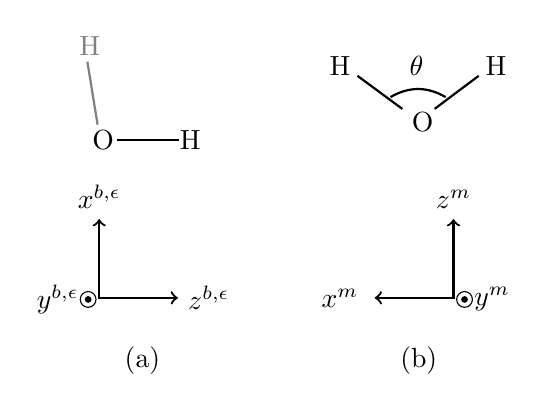
\begin{tikzpicture}[help lines/.style={thin,draw=black!50}]
%\draw[help lines] (0,0) grid (4,4);
%a
\draw [<->,thick] (0,1) node (xaxis) [above] {$x^{\text{b},\epsilon}$}
  |- (1,0) node (zaxis) [right] {$z^{\text{b},\epsilon}$};
  \filldraw[black] (-0.14,-0.02) circle (1pt) node [anchor=east] {$y^{\text{b},\epsilon}$};
\draw(-0.14,-0.02) circle (0.1);
\draw (0.2, -0.8) node [anchor=west] {(a)};
% H2O
\draw[gray,thick] (-0.02, 2.2) coordinate (a_1) -- (-0.15, 3) coordinate (a_2);
\draw[thick] (0.23, 2) coordinate (b_1) -- (1.02, 2) coordinate (b_2);
\draw (0.31, 2) node [anchor=east] {O};
\draw (0.9, 2) node [anchor=west] {H};
\draw[gray] (-0.12, 2.95) node [anchor=south] {H};
%\draw (0.56, 2.61) node {\chemfig{[:-84]H-O-[:0]H}};
%b
\draw [<->,thick] (3.5,0)--(4.5,0) node (xaxis){} 
  |- (4.5,0)--(4.5,1) node (zaxis) [above] {$z^{\text{m}}$};
  \filldraw[black] (4.64, -0.02) circle (1pt) node [anchor=west] {$y^{\text{m}}$};
\draw (2.7, 0) node [anchor=west] {$x^{\text{m}}$};
\draw(4.64,-0.02) circle (0.1);
\draw (3.7, -0.8) node [anchor=west] {(b)};
% H2O
\draw[thick] (3.85, 2.4) coordinate (a_1) -- (3.28, 2.82) coordinate (a_2);
\draw[thick] (4.26, 2.4) coordinate (b_1) -- (4.82, 2.82) coordinate (b_2);
\draw[thick] (3.7,2.55) to [out=30,in=150] (4.4,2.55);
\draw (4.03, 2.7) node [anchor=south] {$\theta$};
\draw (4.37, 2.23) node [anchor=east] {O};
\draw (5.04, 2.7) node [anchor=south] {H};
\draw (3.06, 2.7) node [anchor=south] {H};
%\draw (4.06, 2.61) node {\chemfig{[:-37]H-O-[:37]H}};
\end{tikzpicture}
  \caption{\label{fig:frameworks} The representation of the bond (a) and the molecular (b) frameworks. (from Ref. \cite{Khatib2017})}
\end{figure}

%
We used three different frameworks: the lab framework ($x^{\text{l}},y^{\text{l}},z^{\text{l}}$), the molecular framework 
($x^{\text{m}},y^{\text{m}},z^{\text{m}}$) and the bond framework ($x^{\text{b}},y^{\text{b}},z^{\text{b}}$) (see Fig.\thinspace\ref{fig:frameworks}).
In the lab framework, the $z^{\text{l}}$-axis is perpendicular to the interface. 
The molecular frame will be used to decompose the signal into normal modes of water monomers. 
For the $j$-th molecule, the $z^{\text m}$ axis is along the bisector of the H-O-H angle, the $x^{\text m}$ axis is in the molecular plane, 
and the $y^{\text m}$ axis is out of the molecular plane\cite{Khatib2017}. 

In the bond framework, $z^{\text{b},\epsilon}$ axis is along the bond $\epsilon$ of a molecule, $z^{\text{b},\epsilon}$
is in the molecular plane and $y^{\text{b},\epsilon}$ is out of the molecular plane.
\begin{align}
  \dot{\alpha}^{\text{l},\epsilon} &= {{D}}^{\text{m}}{{D}}^{\text{b},\epsilon}(\frac{\partial{\alpha}^{\text{b}}}{\partial r}\dot
    r^{\epsilon})({D}^{\text{b},\epsilon})^{\text{T}}({D}^{\text{m}})^{\text{T}}, \\ 
    \dot\mu^{\text{l},\epsilon} &= {{D}}^{\text{m}}{{D}}^{\text{b},\epsilon}(\frac{\partial \mu^{\text{b}}}{\partial r}\dot r^{\epsilon}).
    \label{eq:dot_mu-alpha}
 \end{align}
The direction cosine matrix ${{D}}^{\text{b},\epsilon=1}$ and ${{D}}^{\text{b},\epsilon=-1}$ can be expressed as 
\begin{equation}
    {{D}}^{\text{b},1}=\left(
                \begin{matrix}
                    \text{cos}\frac{\theta}{2} &  0  & -\text{sin}\frac{\theta}{2}\\
                    0 & 1 & 0\\
                    \text{sin}\frac{\theta}{2} & 0 & \text{cos}\frac{\theta}{2}
\end{matrix}
\right),\quad
    {{D}}^{\text{b},-1}=\left(
         \begin{matrix}
             -\text{cos}\frac{\theta}{2} & 0 & \text{sin}\frac{\theta}{2}\\
             0 & 1 & 0\\
             \text{sin}\frac{\theta}{2} & 0  & \text{cos}\frac{\theta}{2}
\end{matrix}
\right),
\label{eq:D_b}
\end{equation}
where $\theta$ is the H-O-H angle in a water molecule.
%The approximate value of the angle is 105.5$^\circ$.
We use ${{D}}^{\text{m}}$ to transform the coordinates in a molecular framework to coordinates in the lab framework. 
Because the orientation of water molecules is changing during the simulation, 
%the angle $\theta'_i$ between the water dipole moment and the $z$-axis is time dependent, therefore, 
${{D}}^{\text{m}}$ is time dependent. 
%It can be expressed as 
%\begin{equation}
%    {\bf{D}}^{\text{m}}=
%    \left(
%        \begin{matrix}
%            \text{cos}{\gamma} & \text{sin}{\gamma} & 0\\
%            -\text{sin}{\gamma} & \text{cos}{\gamma} & 0\\
%            0 & 0 & 1
%        \end{matrix}
%     \right)
%     \left(
%         \begin{matrix}
%             \text{cos}{\theta'} & 0 & -\text{sin}{\theta'}\\
%             0 & 1 & 0\\
%             \text{sin}{\theta'} & 0  & \text{cos}{\theta'}
%         \end{matrix}
%     \right) 
%     =
%     \left(
%         \begin{matrix}
%             \text{cos}{\gamma}\text{cos}{\theta'} & \text{sin}{\gamma} & -\text{cos}{\gamma}\text{sin}{\theta'}\\
%             -\text{sin}{\gamma}\text{cos}{\theta'} & \text{cos}{\gamma} & \text{sin}{\gamma}\text{sin}{\theta'}\\
%             \text{sin}{\theta'} & 0  & \text{cos}{\theta'}
%         \end{matrix}
%     \right),
%\label{eq:D_m}
%\end{equation}
%where $\gamma$ is the angle between the incident plane (x-z plane) and the molecular plane of a water molecule,
%and $\theta'$ is the angle of the dipole moment of the water molecule from the normal direction of the interface, 
%and both $\gamma$ and $\theta'$ are time dependent.

Based on DFTMD simulations, we can implement the parameterization of $\frac{\partial \mu_{k}}{\partial r_z}$ and $\frac{\partial\alpha_{ij}}{\partial r_z}$
and calculate the correlation function $\langle\dot{A}_{\eta\xi}(t)\dot{M}_{\kappa}(0)\rangle$ through the velocity auto-correlation function. 
This approximation for estimating the susceptibility retains the details of the interface, including the full electronic structure. 
And it reduces the computational cost for a total calculation with the instantaneous evaluation of the molecular dipoles and polarizabilities\cite{sulpizi2013}. 
The parametrization of $\frac{\partial \mu_{k}}{\partial r_z}$ and $\frac{\partial\alpha_{ij}}{\partial r_z}$ is based 
on the calculation of the MLWF\cite{Marzari97} 
 and can be done through the approach developed by Salanne \etal\cite{Salanne08} and Khatib \etal\cite{Khatib2017}.
The implementation of this parametrization is given in Appendix \ref{calculate_derivatives}.
%\paragraph{Calculation of $\chi^{(2)}$ (Method 2)}
%We now consider the velocities projection on the water normal modes, identified by the collective variables ${\bf{R}}_j$ in the molecular framework. 
%The single water molecule has nine normal modes. Six of them have the angular frequencies $\omega$ equal zero and three normal modes remains. 
%The three normal modes are the symmetric stretching (SS), the antisymmetric stretching (AS) and the bending (B).
%The dipole moment and the molecular polarizability of the $i$th water molecule can be rewritten as
%\begin{align}
%    \dot{\bf \alpha}_{i}^{\text{l}}(t)&={\bf{D}}_{\text{m},i}(\sum_{j=Q,SS,AS}\frac{\partial{\bf\alpha}_{i}^{\text{m}}}{\partial R_j}){\bf{D}}^{\text{T}}_{\text{m},i}, \\ 
%    \dot{\bf \mu}_{i}^{\text{l}}&={\bf{D}}_{\text{m},i}(\sum_{j=Q,SS,AS}\frac{\partial{\bf\mu}_i^{\text{m}}}{\partial R_j}\dot{R}_j).  
%    \label{eq:dot_mu_alpha}
%\end{align}
%where $i$ denote the $i$-th water molecule.
%To parametrize the derivatives $\frac{\partial \alpha_i^{\text{m}}}{\partial R_j}$ and $\frac{\partial {\bf{\mu}}_i^{\text{m}}}{\partial R_j}$,
%the Maximally Localized Wannier Functions (MLWF) were emplyed.\cite{Salanne08,Khatib2017}
\section{Available experimental data}\label{section_SFG_Exp}
In this chapter, we give the experimental results obtained on salty solutions containing alkali cations and nitrate (iodide) anions\cite{PS03,AJ12,HuaWei2014}. 

From the experimental data of surface tension dependence on solute concentration $\text{d}\gamma/\text{d}m_2$ 
at low electrolyte concentrations ($\leq$1.5 M )\cite{Weissenborn95,Hey81,Jarvis68,Jarvis72}, 
the relation of the surface/bulk molar concentration ratio $K_{\text{p}}$\cite{Pegram2006} among \li, \Na and \K is: 
\begin{equation}
0=K_{\text{p,Na}^+}< K_{\text{p,K}^+}< K_{\text{p,Li}^+}.
\label{eq:bscr}
\end{equation}
i.e., \Na is the most surface-excluded in the alkali nitrate solution RNO$_3$, \K is less excluded, 
and \Li is the least excluded cation (see Appendix \ref{surface_tension_increment} for details).
In modeling the interfaces of aqueous solutions of alkali nitrates, we started with LiNO$_3$, 
because the \Li ion is the least excluded of the solution/vapor interface among the alkali metal ions. 

Hua \etal\cite{HuaWei2014} have recently measured the VSFG spectra of water/vapor interface of \LiN salt solutions in the OH stretching region
(3000--3800 \centimeter) using heterodyne detected VSFG spectroscopy\cite{HuaWei2011,HuaWei2011b,ChenXiangKe2010}. 
The experimental result of the VSFG intensity of the alkali nitrate interfaces is given by in Fig.\thinspace\ref{fig:Allen12}. 
At a difference with the spectra for the water/vapor interface, in the spectra of 
\LiN solutions, a depletion of the 3200 \cm peak is observed, with an 
enhancement of the 3400 \cm peak.
A similar behaviour had been observed for the interface of NaNO$_3$ and 
Mg(NO$_3$)$_2$ solutions\cite{AJ12,HuaWei2014}. It has been 
suggested that this depletion of the 3200 \cm peak, and in some cases 
the enhancement of the 3400 \cm peak, is an indication that nitrate 
ions reside at the interface. On the other hand the small 
cations should have little surface propensity. 
It has also been argued that the positive electric field found at the interface of NaCl, NaI and 
NaNO$_3$ salt solutions is due to the formation of an ionic double layer 
between anions located near the surface and their counter-cations (e.g.
Na$^+$) located further below. In Phase-Sensitive (PS) VSFG experiments the 
magnitude of the induced change in the $\Im\chi^{(2)}$ spectra comparatively
to that of the neat water suggested that \nitrate has a surface propensity 
just in between I$^-$ and Cl$^-$\cite{Verreault2013,Verreault2009}. 
% exp. results.
\begin{figure}[H] %[htbp]
\centering
  \includegraphics [width=0.6 \textwidth] {./diagrams/vsfg_alkali_nitrate}
\setlength{\abovecaptionskip}{0pt}
  \caption{\label{fig:Allen12}Experimental VSFG intensity of \LiN solutions, compared with that of neat water\cite{HuaWei2014}.}
\end{figure}
